% A document that is not in the corpus.
%
% The other four examples were written to exercise a compiler; this one was
% written to exercise a *mirror*. `05-SPEC-latex.md` step 3 puts a card in
% front of an author and offers to compile what they have, and what they have
% is not four files chosen by us. So this asks for the four packages an
% ordinary paper asks for and the corpus does not:
%
%   booktabs   a table anyone would write        collection-latexrecommended
%   siunitx    units, in a paper with numbers    collection-mathscience
%   tikz       a figure drawn rather than         collection-pictures
%              included
%   biblatex   the bibliography package that      collection-bibtexextra
%              replaced BibTeX
%
% Two of the four are in the package set the spec's step 3 names and two are
% not, which is the measurement this file exists to make. It compiles on a
% TeX Live on a desk; what it does on SwiftLaTeX pdfTeX against a given mirror
% is the question, and `latex/corpus/MEASUREMENTS.md` records the answer.
\documentclass[11pt]{article}

\begin{filecontents*}[overwrite]{packages.bib}
@article{knuth1984,
  author  = {Knuth, Donald E.},
  title   = {Literate Programming},
  journal = {The Computer Journal},
  volume  = {27},
  number  = {2},
  pages   = {97--111},
  year    = {1984},
}
\end{filecontents*}

\usepackage[T1]{fontenc}
\usepackage{booktabs}
\usepackage{siunitx}
\usepackage{tikz}
\usepackage[backend=bibtex]{biblatex}
\addbibresource{packages.bib}

\title{Four Packages a Paper Asks For}
\author{The Komodoc Corpus}
\date{}

\begin{document}
\maketitle

\section{A table}

\begin{table}[h]
  \centering
  \begin{tabular}{lS[table-format=3.2]S[table-format=1.3]}
    \toprule
    sample & {mass (\si{\gram})} & {error (\si{\gram})} \\
    \midrule
    one   & 102.31 & 0.004 \\
    two   &  98.07 & 0.011 \\
    three & 110.55 & 0.002 \\
    \bottomrule
  \end{tabular}
  \caption{Three masses, set with \texttt{booktabs} and \texttt{siunitx}.}
\end{table}

A quantity written properly is \SI{9.81}{\metre\per\second\squared}, and a
range is \SIrange{1}{10}{\kilo\gram}.

\section{A figure that is drawn}

\begin{figure}[h]
  \centering
  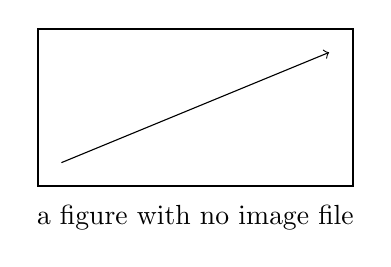
\begin{tikzpicture}
    \draw[thick] (0,0) rectangle (4,2);
    \draw[->] (0.3,0.3) -- (3.7,1.7);
    \node at (2,-0.4) {a figure with no image file};
  \end{tikzpicture}
  \caption{Drawn by \texttt{tikz} rather than included from a file.}
\end{figure}

\section{A bibliography}

Literate programming again~\cite{knuth1984}, so that \texttt{biblatex} has
something to typeset.

\printbibliography

\end{document}
